\documentclass[xcolor=dvipsnames,serif]{beamer}\usepackage[]{graphicx}\usepackage[]{color}
%% maxwidth is the original width if it is less than linewidth
%% otherwise use linewidth (to make sure the graphics do not exceed the margin)
\makeatletter
\def\maxwidth{ %
  \ifdim\Gin@nat@width>\linewidth
    \linewidth
  \else
    \Gin@nat@width
  \fi
}
\makeatother

\definecolor{fgcolor}{rgb}{0.345, 0.345, 0.345}
\newcommand{\hlnum}[1]{\textcolor[rgb]{0.686,0.059,0.569}{#1}}%
\newcommand{\hlstr}[1]{\textcolor[rgb]{0.192,0.494,0.8}{#1}}%
\newcommand{\hlcom}[1]{\textcolor[rgb]{0.678,0.584,0.686}{\textit{#1}}}%
\newcommand{\hlopt}[1]{\textcolor[rgb]{0,0,0}{#1}}%
\newcommand{\hlstd}[1]{\textcolor[rgb]{0.345,0.345,0.345}{#1}}%
\newcommand{\hlkwa}[1]{\textcolor[rgb]{0.161,0.373,0.58}{\textbf{#1}}}%
\newcommand{\hlkwb}[1]{\textcolor[rgb]{0.69,0.353,0.396}{#1}}%
\newcommand{\hlkwc}[1]{\textcolor[rgb]{0.333,0.667,0.333}{#1}}%
\newcommand{\hlkwd}[1]{\textcolor[rgb]{0.737,0.353,0.396}{\textbf{#1}}}%
\let\hlipl\hlkwb

\usepackage{framed}
\makeatletter
\newenvironment{kframe}{%
 \def\at@end@of@kframe{}%
 \ifinner\ifhmode%
  \def\at@end@of@kframe{\end{minipage}}%
  \begin{minipage}{\columnwidth}%
 \fi\fi%
 \def\FrameCommand##1{\hskip\@totalleftmargin \hskip-\fboxsep
 \colorbox{shadecolor}{##1}\hskip-\fboxsep
     % There is no \\@totalrightmargin, so:
     \hskip-\linewidth \hskip-\@totalleftmargin \hskip\columnwidth}%
 \MakeFramed {\advance\hsize-\width
   \@totalleftmargin\z@ \linewidth\hsize
   \@setminipage}}%
 {\par\unskip\endMakeFramed%
 \at@end@of@kframe}
\makeatother

\definecolor{shadecolor}{rgb}{.97, .97, .97}
\definecolor{messagecolor}{rgb}{0, 0, 0}
\definecolor{warningcolor}{rgb}{1, 0, 1}
\definecolor{errorcolor}{rgb}{1, 0, 0}
\newenvironment{knitrout}{}{} % an empty environment to be redefined in TeX

\usepackage{alltt}
\usetheme{Boadilla}
\usecolortheme[named=CornflowerBlue]{structure}
\usepackage{graphicx}
\usepackage{breqn}
\usepackage{xcolor}
\usepackage{booktabs}
\usepackage{verbatim}
\usepackage{tikz}
\usepackage[final]{animate}
\usepackage{lmodern}
\usetikzlibrary{shadows,arrows,positioning}
\definecolor{links}{HTML}{2A1B81}
\hypersetup{colorlinks,linkcolor=links,urlcolor=links}
\usepackage{pgfpages}

\tikzstyle{block} = [rectangle, draw, text width=9em, text centered, rounded corners, minimum height=3em, minimum width=7em, top color = white, bottom color=brown!30,  drop shadow]

% change font of frame titles and title slide
\setbeamerfont{title}{series=\bfseries}
\setbeamerfont{frametitle}{series=\bfseries} 

% enumerate style
\setbeamertemplate{enumerate items}[circle]

% my macros
\newcommand{\ShowSexpr}[1]{\texttt{{\char`\\}Sexpr\{#1\}}}
\newcommand{\Bigtxt}[1]{\textbf{\textit{#1}}}
\IfFileExists{upquote.sty}{\usepackage{upquote}}{}
\begin{document}

\title[TS decomposition]{Time series topic 2: Decomposition}

\author[M. Beck]{Marcus W. Beck\inst{1}}

\date{}

\institute[]{\inst{1} USEPA NHEERL Gulf Ecology Division\\ Email: \href{mailto:beck.marcus@epa.gov}{beck.marcus@epa.gov}}

% knitr setup


% dependents


% get online bib file


%%%%%%
\begin{frame}
\vspace{0.3in}
\centerline{
\begin{tikzpicture}
  \node[drop shadow={shadow xshift=0ex,shadow yshift=0ex},fill=white,draw] at (0,0) {
\includegraphics[width=0.9\textwidth]{imgs/workshop2016logo.png}};
\end{tikzpicture}}
\titlepage
\end{frame}

\section{Overview}

%%%%%%
\begin{frame}{Objectives for the session (3:30-4:15)}
\begin{itemize}
\item What is and why do we use time series decomposition \\~\\
\item Functions in SWMPr \\~\\
\item Application to NERRS data \\~\\
\begin{itemize}
\item Data prep \\~\\
\item Execution \\~\\
\item Interpretation 
\end{itemize}
\end{itemize}
\end{frame}

%%%%%%
\begin{frame}{Interactive portion}
\onslide<+->
Follow along as we go:\\~\\
\begin{itemize}
\item flash drive\\~\\
\item online: \href{http://swmprats.net/}{swmprats.net} 2016 workshop tab \\~\\
\end{itemize}
\onslide<+->
You will run examples whenever you see this guy: \\~\\
\centerline{
\includegraphics[width = 0.15\textwidth]{imgs/swmprat.png}} 
\end{frame}

%%%%%%
\begin{frame}[fragile]{
\includegraphics[width = 0.05\textwidth]{imgs/swmprat.png} Is everything installed?}
\onslide<1->
We will use functions in the SWMPr package \\~\\
Option 1, from the R Console prompt:
\begin{knitrout}\scriptsize
\definecolor{shadecolor}{rgb}{0.969, 0.969, 0.969}\color{fgcolor}\begin{kframe}
\begin{alltt}
\hlkwd{install.packages}\hlstd{(}\hlstr{'SWMPr'}\hlstd{)}
\hlkwd{library}\hlstd{(SWMPr)}
\end{alltt}
\end{kframe}
\end{knitrout}
\onslide<2->
\vspace{0.1in}
Option 2, install the source file from the flash drive:
\begin{knitrout}\scriptsize
\definecolor{shadecolor}{rgb}{0.969, 0.969, 0.969}\color{fgcolor}\begin{kframe}
\begin{alltt}
\hlcom{# change as needed}
\hlstd{path_to_file} \hlkwb{<-} \hlstr{'C:/Users/mbeck/Desktop/SWMPr_2.2.0.tar.gz'}

\hlcom{# install, load}
\hlkwd{install.packages}\hlstd{(path_to_file,} \hlkwc{repos} \hlstd{=} \hlkwa{NULL}\hlstd{,} \hlkwc{type}\hlstd{=}\hlstr{"source"}\hlstd{)}
\hlkwd{library}\hlstd{(SWMPr)}
\end{alltt}
\end{kframe}
\end{knitrout}
\end{frame}



%%%%%%
\begin{frame}[t]{Theory and background}{}
{\bf \centerline{Observed data represents effects of many processes}}
\vspace{0.15in}
\centerline{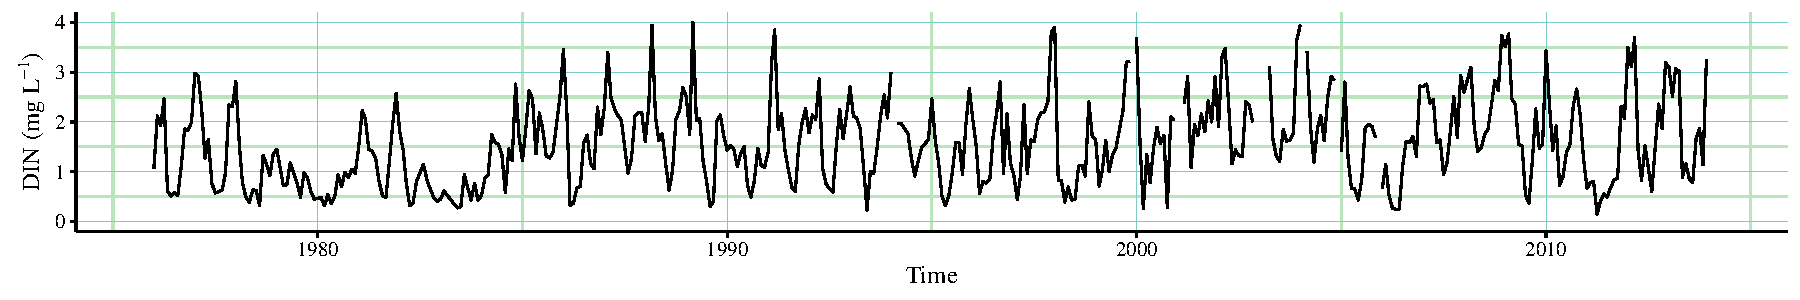
\includegraphics[width = \textwidth]{imgs/ts_ex.pdf}}
\vspace{0.15in}
\begin{columns}[t]
\begin{column}{0.3\textwidth}
{\bf \underline{\Bigtxt{Climate}}}\\
precipitation\\
temperature\\
wind events\\
ENSO effects
\end{column}
\begin{column}{0.3\textwidth}
{\bf \underline{\Bigtxt{Local}}}\\
light/turbidity\\
residence time\\
invasive species\\
trophic effects
\end{column}
\begin{column}{0.3\textwidth}
{\bf \underline{\Bigtxt{Regional/historical}}}\\
watershed inputs\\
point sources\\
management actions
flow changes
\end{column}
\end{columns}
\end{frame}

%%%%%%
\begin{frame}[t]{Theory and background}
\onslide<+->
{\bf \centerline{Observed data represents effects of many processes}}
\vspace{0.15in}
\centerline{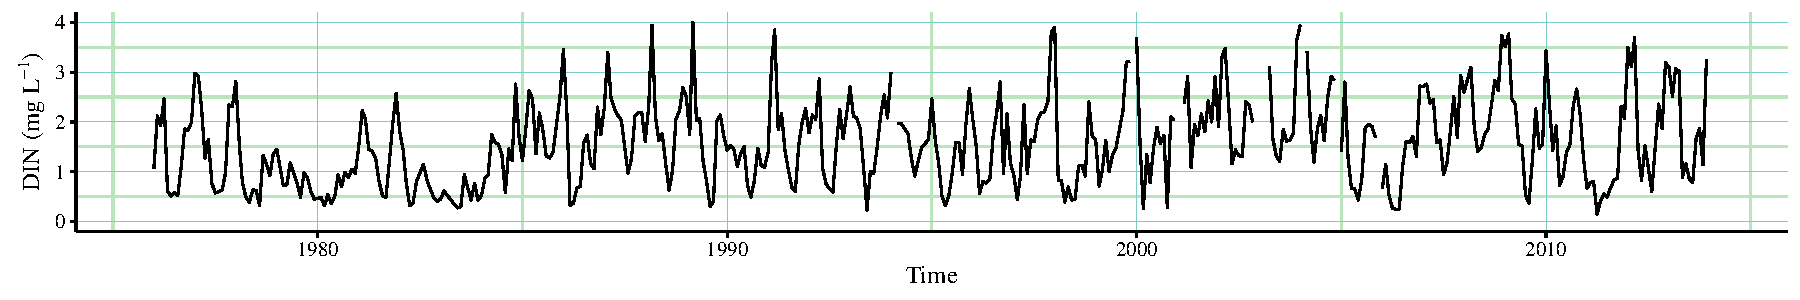
\includegraphics[width = \textwidth]{imgs/ts_ex.pdf}}
\centerline{Models should describe components to evaluate effects}
\vspace{-0.1in}
\begin{columns}[t]
\begin{column}{0.5\textwidth}
\onslide<+->{
\centerline{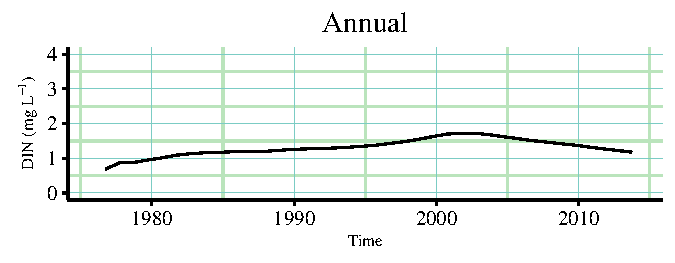
\includegraphics[width = 0.8\textwidth]{imgs/schematic2.pdf}}
\centerline{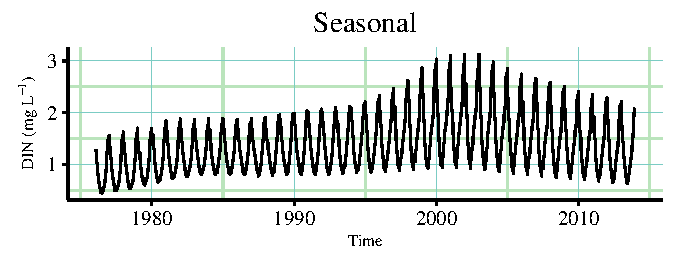
\includegraphics[width = 0.8\textwidth]{imgs/schematic3.pdf}}
}
\end{column}
\begin{column}{0.5\textwidth}
\onslide<+->{
\centerline{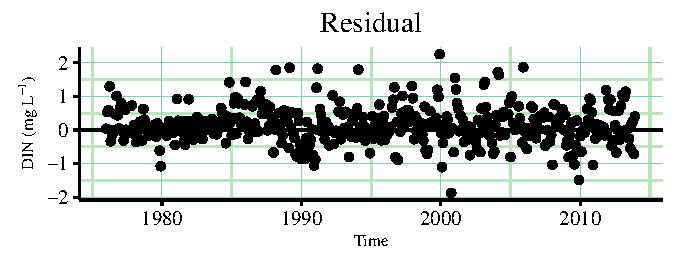
\includegraphics[width = 0.8\textwidth]{imgs/schematic4.pdf}}
\centerline{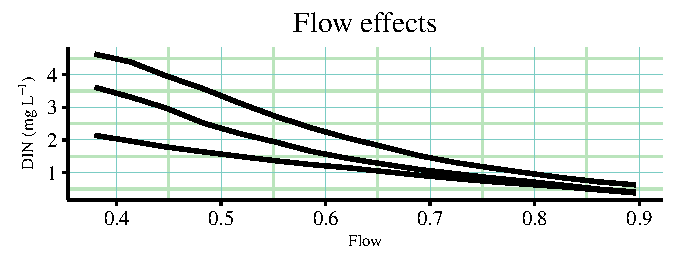
\includegraphics[width = 0.8\textwidth]{imgs/schematic5.pdf}}
}
\end{column}
\end{columns}
\end{frame}

%%%%%%
\begin{frame}{Theory and background}
\begin{itemize}
\item<1-> Time series decomposition is a very general topic - WRTDS is a form of decomposition \\~\\
\item<2-> There are more generic and simpler approaches \\~\\
\item<3-> Objective is to decompose a time series into individual components, isolate or otherwise remove components of interests \\~\\
\item<4-> The individual components are sometimes additive or multiplicative components of the complete time series \\~\\
\item<5-> But be warned... just because you can doesn't mean you should
\end{itemize}
\end{frame}

%%%%%%
\begin{frame}[t]{Theory and background}
\onslide<1->
Two very general decomposition methods are provided in SWMPr: \texttt{decomp()} and \texttt{decomp_cj} \\~\\
These are not new methods, they just make it easy to decompose NERRS data - work with swmpr objects \\~\\
\begin{columns}[t]
\begin{column}{\textwidth}
\onslide<2->
\underline{\texttt{decomp()}} \\~\\
\begin{itemize}
\item<2-> Almost identical to the \texttt{decompose} function
\item<3-> Works well for time series with daily or seasonal cycles
\item<4-> Separates components as trend, cyclical variation (e.g., annual, daily), and random
\item<5-> Additive or multiplicative decomposition
\end{itemize}
\end{column}
\end{columns}
\end{frame}

%%%%%%
\begin{frame}[t]{Theory and background}
\onslide<1->
Two very general decomposition methods are provided in SWMPr: \texttt{decomp()} and \texttt{decomp_cj} \\~\\
These are not new methods, they just make it easy to decompose NERRS data - work with swmpr objects \\~\\
\begin{columns}[t]
\begin{column}{\textwidth}
\underline{\texttt{decomp()}} \\~\\
\begin{enumerate}
\item Gets trend by moving average, removes it from the time series.
\item<2-> Gets seasonal variation by averaging across time periods
\item<3-> Gets error as the remainder from the trend and seasonal components
\end{enumerate}
\end{column}
\end{columns}
\end{frame}

%%%%%%
\begin{frame}[t]{Theory and background}
\onslide<1->
Two very general decomposition methods are provided in SWMPr: \texttt{decomp()} and \texttt{decomp_cj} \\~\\
These are not new methods, they just make it easy to decompose NERRS data - work with swmpr objects  \\~\\
\begin{columns}[t]
\begin{column}{\textwidth}
\underline{\texttt{decomp_cj()}}\\~\\
\begin{itemize}
\item Based on a deprecated method in the wq package, described in \cite{Cloern10}
\item<2-> Works only for time series with seasonal cycles
\item<3-> Separates components as grandmean, annual, seasonal, and events
\item<4-> Additive or multiplicative decomposition
\end{itemize}
\end{column}
\end{columns}
\end{frame}

%%%%%%
\begin{frame}[t]{Theory and background}
\onslide<1->
Two very general decomposition methods are provided in SWMPr: \texttt{decomp()} and \texttt{decomp_cj} \\~\\
These are not new methods, they just make it easy to decompose NERRS data - work with swmpr objects  \\~\\
\begin{columns}[t]
\begin{column}{\textwidth}
\underline{\texttt{decomp_cj()}}\\~\\
\begin{enumerate}
\item Takes grandmean, removes it from time series
\item<2-> Annual trends as averages within years, removes from time series
\item<3-> Seasonal trend as averages between periods, removes from time series
\item<4-> Events as remainder
\end{enumerate}
\end{column}
\end{columns}
\end{frame}

\section{Application}

%%%%%%
\begin{frame}[fragile]{
\includegraphics[width = 0.05\textwidth]{imgs/swmprat.png} Using \texttt{decomp} with NERRS data}
Load some water quality data from Apalachicola Bay, Dry Bar station \\~\\
Let's look at DO variation over one month
\begin{knitrout}\scriptsize
\definecolor{shadecolor}{rgb}{0.969, 0.969, 0.969}\color{fgcolor}\begin{kframe}
\begin{alltt}
\hlcom{# load SWMPr}
\hlkwd{library}\hlstd{(SWMPr)}

\hlcom{# subset for daily decomposition}
\hlstd{dat} \hlkwb{<-} \hlkwd{subset}\hlstd{(apadbwq,} \hlkwc{subset} \hlstd{=} \hlkwd{c}\hlstd{(}\hlstr{'2013-07-01 00:00'}\hlstd{,} \hlstr{'2013-07-31 00:00'}\hlstd{),}
  \hlkwc{select} \hlstd{=} \hlstr{'do_mgl'}\hlstd{)}
\hlkwd{plot}\hlstd{(dat)}
\end{alltt}
\end{kframe}

{\centering 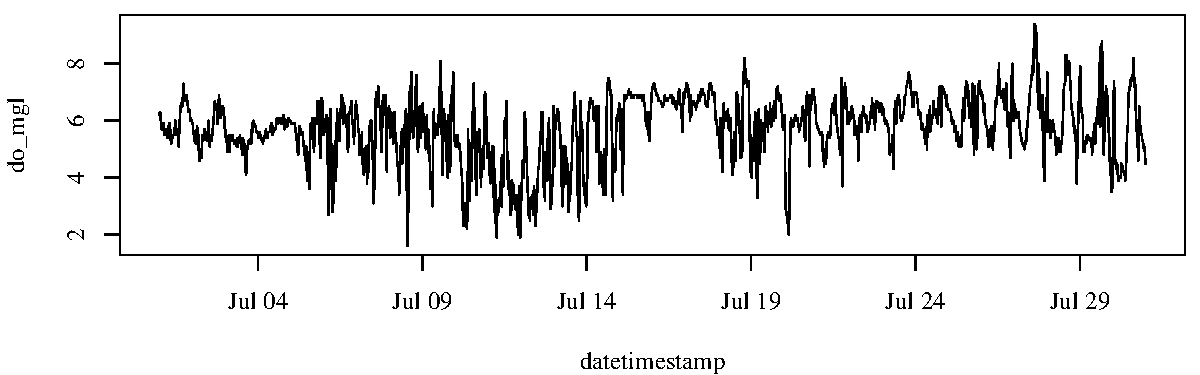
\includegraphics[width=\maxwidth]{imgs/dailyobs-1} 

}



\end{knitrout}
\end{frame}

%%%%%%
\begin{frame}[fragile]{
\includegraphics[width = 0.05\textwidth]{imgs/swmprat.png} Using \texttt{decomp} with NERRS data}
\begin{knitrout}\scriptsize
\definecolor{shadecolor}{rgb}{0.969, 0.969, 0.969}\color{fgcolor}\begin{kframe}
\begin{alltt}
\hlstd{dat_add} \hlkwb{<-} \hlkwd{decomp}\hlstd{(dat,} \hlkwc{param} \hlstd{=} \hlstr{'do_mgl'}\hlstd{,} \hlkwc{frequency} \hlstd{=} \hlstr{'daily'}\hlstd{,} \hlkwc{type} \hlstd{=} \hlstr{'additive'}\hlstd{)}
\hlkwd{plot}\hlstd{(dat_add)}
\end{alltt}
\end{kframe}

{\centering 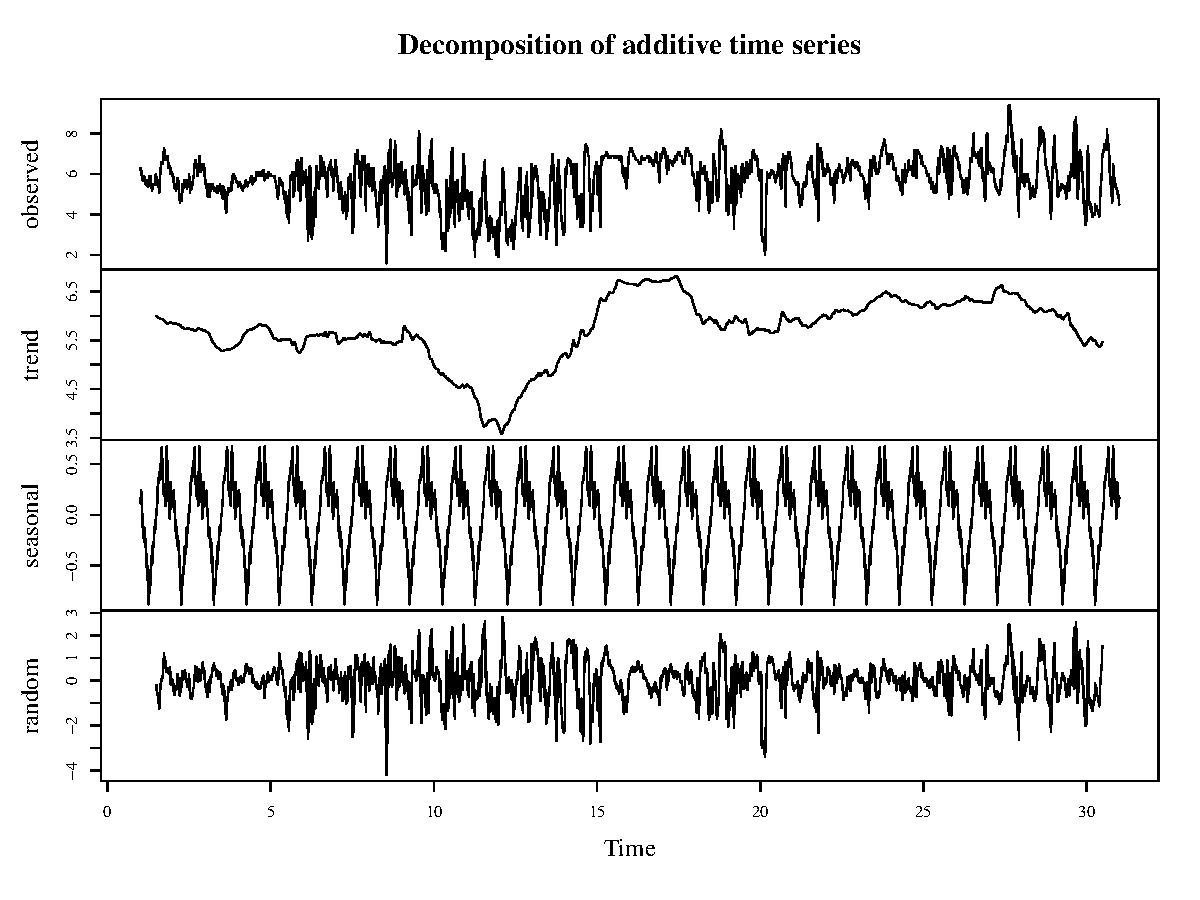
\includegraphics[width=0.7\textwidth]{imgs/dailydcadd-1} 

}



\end{knitrout}
\end{frame}

%%%%%%
\begin{frame}[fragile]{
\includegraphics[width = 0.05\textwidth]{imgs/swmprat.png} Using \texttt{decomp} with NERRS data}
What's in the decomposed object?  
\begin{knitrout}\scriptsize
\definecolor{shadecolor}{rgb}{0.969, 0.969, 0.969}\color{fgcolor}\begin{kframe}
\begin{alltt}
\hlkwd{str}\hlstd{(dat_add)}
\end{alltt}
\begin{verbatim}
## List of 6
##  $ x       : Time-Series [1:2881] from 1 to 31: 6.2 6.3 6.3 6.2 6 5.9 5.7 5.8 5.7 5.7 ...
##  $ seasonal: Time-Series [1:2881] from 1 to 31: 0.165 0.12 0.178 0.239 0.163 ...
##  $ trend   : Time-Series [1:2881] from 1 to 31: NA NA NA NA NA NA NA NA NA NA ...
##  $ random  : Time-Series [1:2881] from 1 to 31: NA NA NA NA NA NA NA NA NA NA ...
##  $ figure  : num [1:96] 0.165 0.12 0.178 0.239 0.163 ...
##  $ type    : chr "additive"
##  - attr(*, "class")= chr "decomposed.ts"
\end{verbatim}
\begin{alltt}
\hlkwd{str}\hlstd{(dat_add}\hlopt{$}\hlstd{trend)}
\end{alltt}
\begin{verbatim}
##  Time-Series [1:2881] from 1 to 31: NA NA NA NA NA NA NA NA NA NA ...
\end{verbatim}
\end{kframe}
\end{knitrout}
\end{frame}

%%%%%%
\begin{frame}[fragile]{
\includegraphics[width = 0.05\textwidth]{imgs/swmprat.png} Using \texttt{decomp} with NERRS data}
What does additive mean?
\begin{knitrout}\scriptsize
\definecolor{shadecolor}{rgb}{0.969, 0.969, 0.969}\color{fgcolor}\begin{kframe}
\begin{alltt}
\hlstd{add} \hlkwb{<-} \hlkwd{with}\hlstd{(dat_add, seasonal} \hlopt{+} \hlstd{trend} \hlopt{+} \hlstd{random)}
\hlkwd{plot}\hlstd{(add, dat}\hlopt{$}\hlstd{do_mgl)}
\end{alltt}
\end{kframe}

{\centering 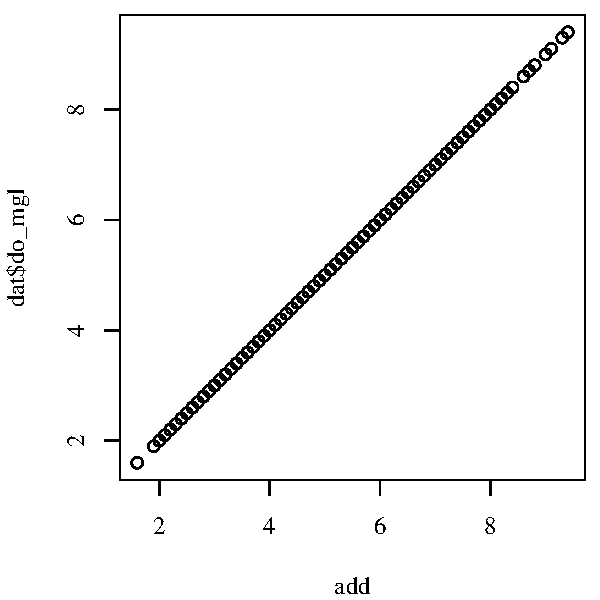
\includegraphics[width=0.5\textwidth]{imgs/dailydc_rcadd-1} 

}



\end{knitrout}
\end{frame}

%%%%%%
\begin{frame}[fragile]{
\includegraphics[width = 0.05\textwidth]{imgs/swmprat.png} Using \texttt{decomp} with NERRS data}
Let's try a multiplicative decomposition
\begin{knitrout}\scriptsize
\definecolor{shadecolor}{rgb}{0.969, 0.969, 0.969}\color{fgcolor}\begin{kframe}
\begin{alltt}
\hlstd{dat_mul} \hlkwb{<-} \hlkwd{decomp}\hlstd{(dat,} \hlkwc{param} \hlstd{=} \hlstr{'do_mgl'}\hlstd{,} \hlkwc{frequency} \hlstd{=} \hlstr{'daily'}\hlstd{,}
  \hlkwc{type} \hlstd{=} \hlstr{'multiplicative'}\hlstd{)}
\hlkwd{plot}\hlstd{(dat_mul)}
\end{alltt}
\end{kframe}

{\centering 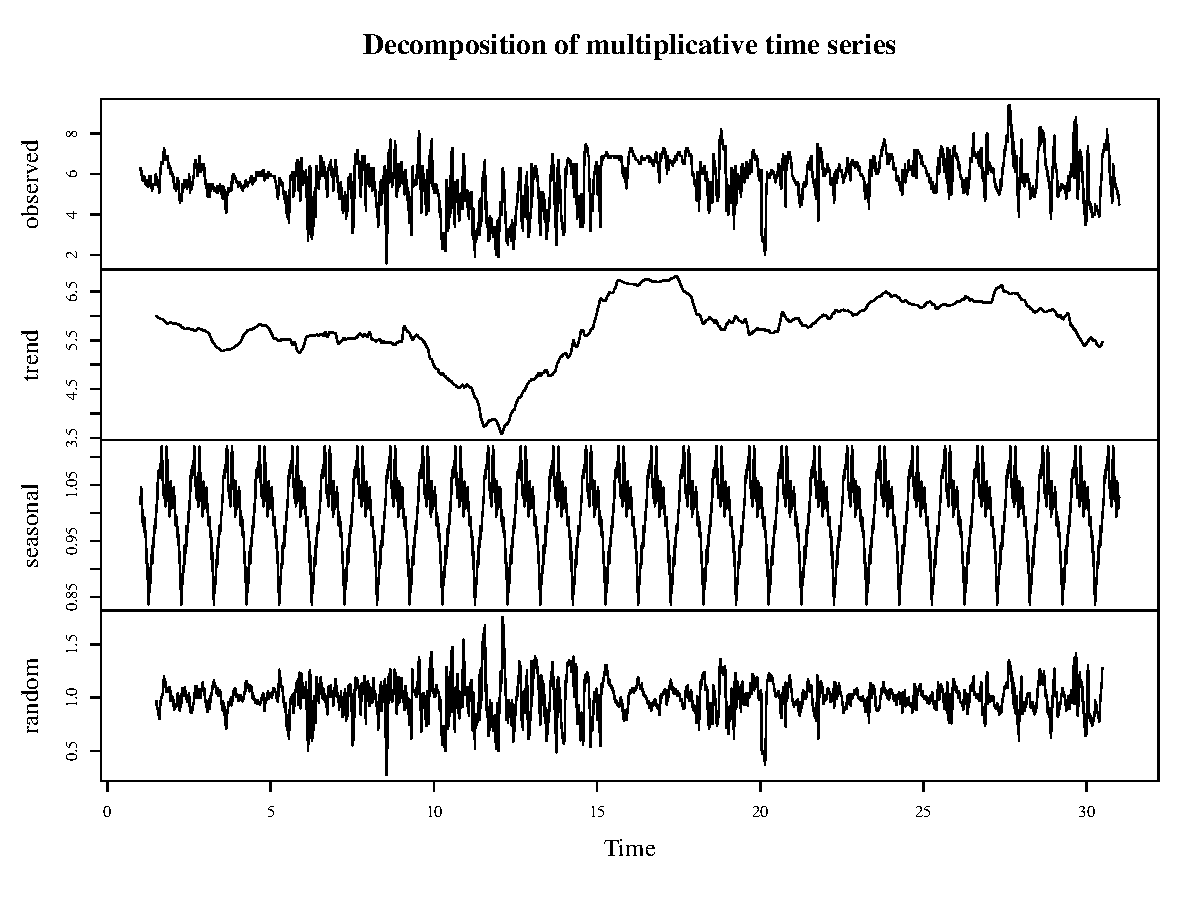
\includegraphics[width=0.7\textwidth]{imgs/dailydcmul-1} 

}



\end{knitrout}
\end{frame}

%%%%%%
\begin{frame}[fragile]{
\includegraphics[width = 0.05\textwidth]{imgs/swmprat.png} Using \texttt{decomp} with NERRS data}
What does multiplicative mean?
\begin{knitrout}\scriptsize
\definecolor{shadecolor}{rgb}{0.969, 0.969, 0.969}\color{fgcolor}\begin{kframe}
\begin{alltt}
\hlstd{mul} \hlkwb{<-} \hlkwd{with}\hlstd{(dat_mul, seasonal} \hlopt{*} \hlstd{trend} \hlopt{*} \hlstd{random)}
\hlkwd{plot}\hlstd{(mul, dat}\hlopt{$}\hlstd{do_mgl)}
\end{alltt}
\end{kframe}

{\centering 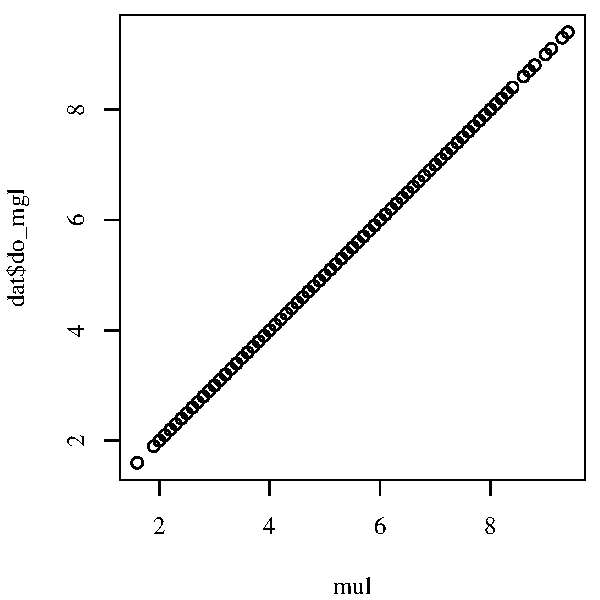
\includegraphics[width=0.5\textwidth]{imgs/dailydc_rcmul-1} 

}



\end{knitrout}
\end{frame}

%%%%%%
\begin{frame}[fragile]{
\includegraphics[width = 0.05\textwidth]{imgs/swmprat.png} Using \texttt{decomp\_cj} with NERRS data}
Use discrete, monthly data with \texttt{decomp\_cj}: Apalachicola Bay, Cat Point nutrient station
\begin{knitrout}\scriptsize
\definecolor{shadecolor}{rgb}{0.969, 0.969, 0.969}\color{fgcolor}\begin{kframe}
\begin{alltt}
\hlstd{apacpnut} \hlkwb{<-} \hlkwd{qaqc}\hlstd{(apacpnut,} \hlkwc{qaqc_keep} \hlstd{=} \hlkwd{c}\hlstd{(}\hlnum{0}\hlstd{,} \hlnum{4}\hlstd{))}
\hlkwd{decomp_cj}\hlstd{(apacpnut,} \hlkwc{param} \hlstd{=} \hlstr{'chla_n'}\hlstd{,} \hlkwc{type} \hlstd{=} \hlstr{'add'}\hlstd{)}
\end{alltt}
\end{kframe}

{\centering 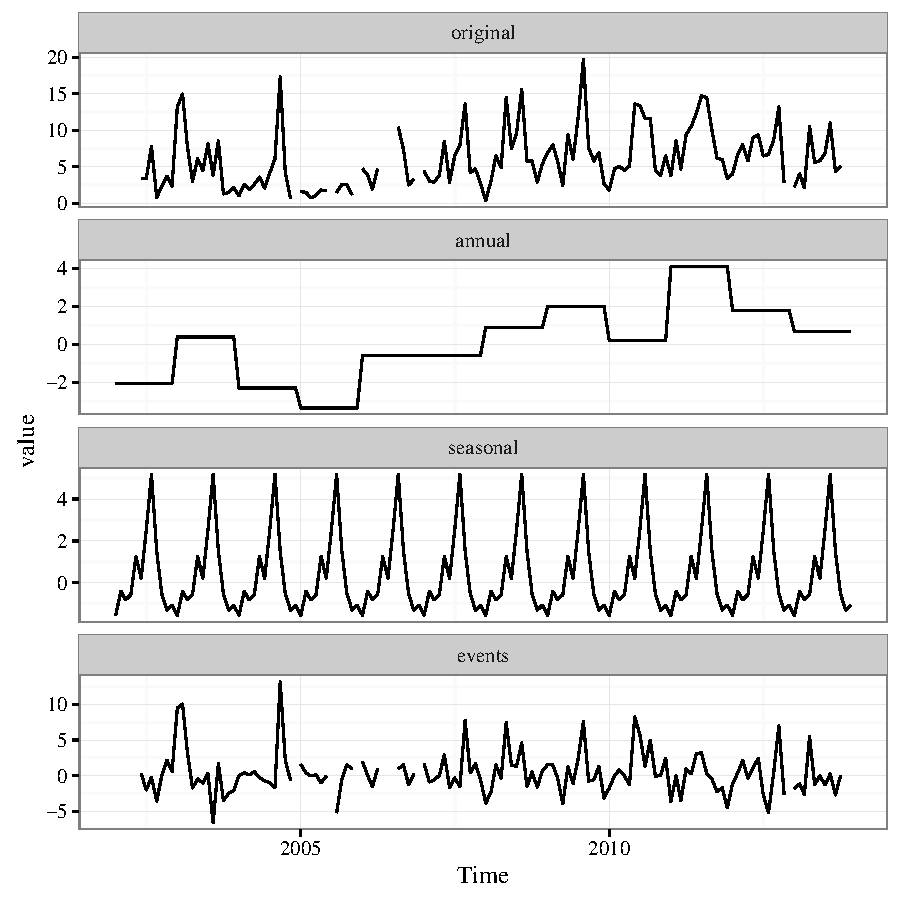
\includegraphics[width=0.5\textwidth]{imgs/monthlydc-1} 

}



\end{knitrout}
\end{frame}

%%%%%%
\begin{frame}[fragile]{
\includegraphics[width = 0.05\textwidth]{imgs/swmprat.png} Using \texttt{decomp\_cj} with NERRS data}
Note that the default behavior for \texttt{decomp\_cj} is a plot, use \texttt{vals\_out = TRUE} for values
\begin{knitrout}\scriptsize
\definecolor{shadecolor}{rgb}{0.969, 0.969, 0.969}\color{fgcolor}\begin{kframe}
\begin{alltt}
\hlstd{add} \hlkwb{<-} \hlkwd{decomp_cj}\hlstd{(apacpnut,} \hlkwc{param} \hlstd{=} \hlstr{'chla_n'}\hlstd{,} \hlkwc{type} \hlstd{=} \hlstr{'add'}\hlstd{,} \hlkwc{vals_out} \hlstd{=} \hlnum{TRUE}\hlstd{)}
\hlkwd{head}\hlstd{(add)}
\end{alltt}
\begin{verbatim}
##         Time original    grand    annual   seasonal     events
## 1 2002-01-01       NA 5.929384 -2.760634 -1.9742526         NA
## 2 2002-02-01       NA 5.929384 -2.760634 -0.4467677         NA
## 3 2002-03-01       NA 5.929384 -2.760634 -1.6590556         NA
## 4 2002-04-01      1.6 5.929384 -2.760634 -1.2348774 -0.3338726
## 5 2002-05-01       NA 5.929384 -2.760634  1.3020742         NA
## 6 2002-06-01      3.4 5.929384 -2.760634  0.4469690 -0.2157190
\end{verbatim}
\end{kframe}
\end{knitrout}
\end{frame}

%%%%%%
\begin{frame}[fragile]{
\includegraphics[width = 0.05\textwidth]{imgs/swmprat.png} Using \texttt{decomp\_cj} with NERRS data}
A word of caution, \texttt{decomp\_cj} uses \texttt{setstep} before decomposing
\begin{knitrout}\scriptsize
\definecolor{shadecolor}{rgb}{0.969, 0.969, 0.969}\color{fgcolor}\begin{kframe}
\begin{alltt}
\hlkwd{head}\hlstd{(apacpnut)}
\end{alltt}
\begin{verbatim}
##         datetimestamp  po4f  nh4f  no2f  no3f no23f chla_n
## 1 2002-04-02 11:55:00 0.004 0.027 0.002 0.048 0.050    1.8
## 2 2002-04-02 11:56:00 0.004 0.029 0.002 0.046 0.048    1.8
## 3 2002-04-30 11:15:00 0.014 0.138 0.005 0.115 0.120    1.2
## 4 2002-06-04 11:03:00 0.006 0.049 0.002 0.024 0.026    3.4
## 5 2002-07-02 09:53:00 0.014 0.083 0.002    NA 0.039    3.7
## 6 2002-07-02 09:55:00 0.017 0.093 0.002    NA 0.040    3.0
\end{verbatim}
\begin{alltt}
\hlkwd{head}\hlstd{(add)}
\end{alltt}
\begin{verbatim}
##         Time original    grand    annual   seasonal     events
## 1 2002-01-01       NA 5.929384 -2.760634 -1.9742526         NA
## 2 2002-02-01       NA 5.929384 -2.760634 -0.4467677         NA
## 3 2002-03-01       NA 5.929384 -2.760634 -1.6590556         NA
## 4 2002-04-01      1.6 5.929384 -2.760634 -1.2348774 -0.3338726
## 5 2002-05-01       NA 5.929384 -2.760634  1.3020742         NA
## 6 2002-06-01      3.4 5.929384 -2.760634  0.4469690 -0.2157190
\end{verbatim}
\end{kframe}
\end{knitrout}
\end{frame}

\section{Summary}

%%%%%%
\begin{frame}[fragile]{
\includegraphics[width = 0.05\textwidth]{imgs/swmprat.png} Summary}{}
A word of caution, \texttt{decomp} does not work with missing data
\begin{knitrout}\scriptsize
\definecolor{shadecolor}{rgb}{0.969, 0.969, 0.969}\color{fgcolor}\begin{kframe}
\begin{alltt}
\hlstd{dat} \hlkwb{<-} \hlkwd{subset}\hlstd{(apadbwq,} \hlkwc{subset} \hlstd{=} \hlkwd{c}\hlstd{(}\hlstr{'2013-06-01 00:00'}\hlstd{,} \hlstr{'2013-07-31 00:00'}\hlstd{))}

\hlcom{# this returns an error}
\hlstd{test} \hlkwb{<-} \hlkwd{decomp}\hlstd{(dat,} \hlkwc{param} \hlstd{=} \hlstr{'do_mgl'}\hlstd{,} \hlkwc{frequency} \hlstd{=} \hlstr{'daily'}\hlstd{)}
\end{alltt}


{\ttfamily\noindent\bfseries\color{errorcolor}{\#\# Error in na.omit.ts(x): time series contains internal NAs}}\end{kframe}
\end{knitrout}
\end{frame}

%%%%%%
\begin{frame}[fragile]{
\includegraphics[width = 0.05\textwidth]{imgs/swmprat.png} Summary}{}
\begin{knitrout}\scriptsize
\definecolor{shadecolor}{rgb}{0.969, 0.969, 0.969}\color{fgcolor}\begin{kframe}
\begin{alltt}
\hlcom{# use na.approx to interpolate missing data}
\hlstd{dat} \hlkwb{<-} \hlkwd{subset}\hlstd{(apadbwq,} \hlkwc{subset} \hlstd{=} \hlkwd{c}\hlstd{(}\hlstr{'2013-06-01 00:00'}\hlstd{,} \hlstr{'2013-07-31 00:00'}\hlstd{))}
\hlstd{dat} \hlkwb{<-} \hlkwd{na.approx}\hlstd{(dat,} \hlkwc{params} \hlstd{=} \hlstr{'do_mgl'}\hlstd{,} \hlkwc{maxgap} \hlstd{=} \hlnum{10}\hlstd{)}

\hlcom{# decomposition and plot}
\hlstd{dat_fl} \hlkwb{<-} \hlkwd{decomp}\hlstd{(dat,} \hlkwc{param} \hlstd{=} \hlstr{'do_mgl'}\hlstd{,} \hlkwc{frequency} \hlstd{=} \hlstr{'daily'}\hlstd{)}
\hlkwd{plot}\hlstd{(dat_fl)}
\end{alltt}
\end{kframe}

{\centering 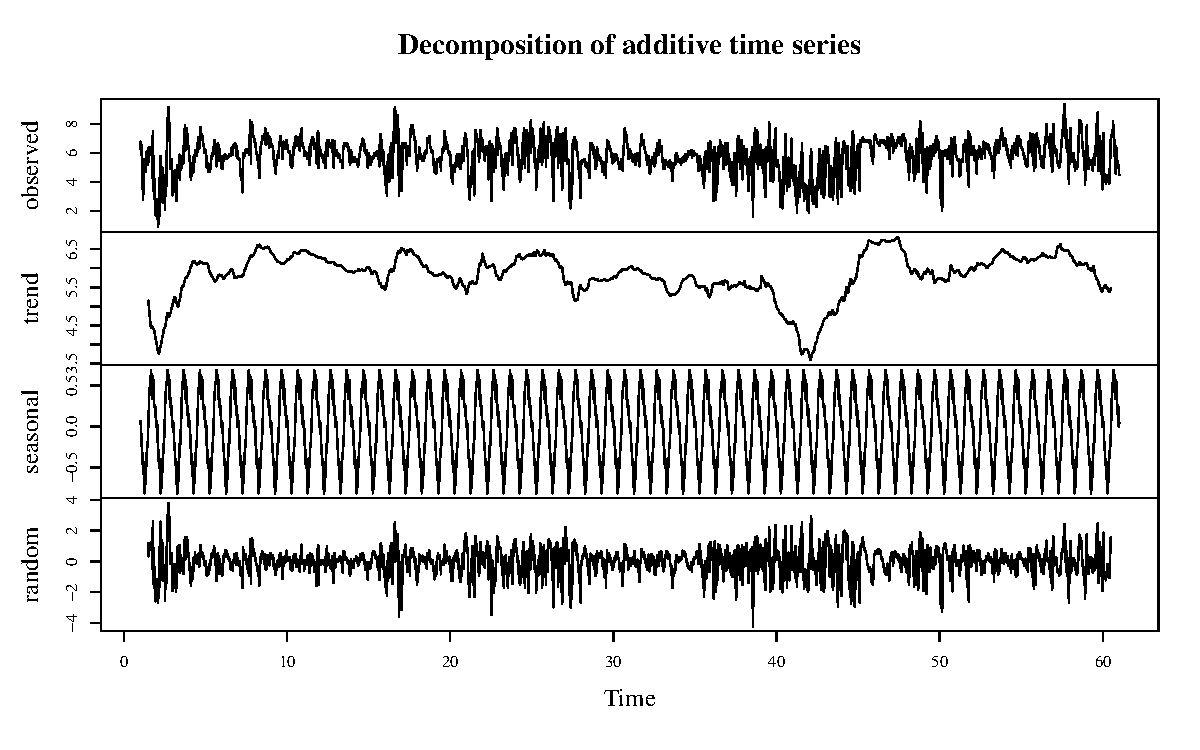
\includegraphics[width=0.7\textwidth]{imgs/dailyfl-1} 

}



\end{knitrout}
\end{frame}

%%%%%%
\begin{frame}{Summary}{}
\onslide<1->
Things to ask before decomposition: \\~\\
\begin{itemize}
\item<1-> What is the time step? Is it regular? Does it need be standardized?
\item<2-> How do I deal with missing data?
\item<3-> Is there any expected cyclical variation? If so, what is the period (e.g., seasonal, daily)?
\item<4-> Is stationarity a reasonable expectation of the cyclical variation (yes = additive, no = multiplicative)?
\end{itemize}
\end{frame}

%%%%%%
\begin{frame}
\vspace{0.3in}
\centerline{
\begin{tikzpicture}
  \node[drop shadow={shadow xshift=0ex,shadow yshift=0ex},fill=white,draw] at (0,0) {
\includegraphics[width=0.9\textwidth]{imgs/workshop2016logo.png}};
\end{tikzpicture}}
\vspace{0.5in}
\centerline{Up next... Time Series Topic 3: Seasonal Kendall}
\vspace{0.5in}
\Large
\centerline{\Bigtxt{Questions??}}
\end{frame}

%%%%%%
\section{References}
\begin{frame}[t]{\textbf{References}}
\tiny
\setbeamertemplate{bibliography item}{}
\bibliographystyle{apalike_mine}
\bibliography{refs}
\end{frame}
\end{document}
